\documentclass{VUMIFInfKursinis}
\usepackage{algorithmicx}
\usepackage{algorithm}
\usepackage{algpseudocode}
\usepackage{amsfonts}
\usepackage{amsmath}
\usepackage{bm}
\usepackage{color}
\usepackage{graphicx}
% \usepackage{hyperref}  % Nuorodų aktyvavimas
\usepackage{url}

\usepackage{gensymb}
\usepackage{acro}
\usepackage{tikz}
\usetikzlibrary{decorations.pathreplacing}
\usepackage{amssymb,amsthm}
\usepackage[version=4]{mhchem}

\setlength{\jot}{8px} 

% Titulinio aprašas
\university{Vilniaus universitetas}
\faculty{Matematikos ir informatikos fakultetas}
\institute{Informatikos institutas}  % Užkomentavus šią eilutę - institutas neįtraukiamas į titulinį
\department{Programų sistemų katedra}
\papertype{Kursinis darbas}
\title{Medžiagų maišymo modeliavimas cheminėse
reakcijose}
\titleineng{Modelling the mixing of reagents in
chemical reactions}
\status{4 kurso 3 grupės studentas}
\author{Arnas Vaicekauskas}
% \secondauthor{Vardonis Pavardonis}   % Pridėti antrą autorių
\supervisor{Asist. Dr. Rokas Astrauskas}
\date{Vilnius \\ \the\year}

% Nustatymai
% \setmainfont{Palemonas}   % Pakeisti teksto šriftą į Palemonas (turi būti įdiegtas sistemoje)
\bibliography{bibliografija} 

\DeclareAcronym{yag}{
  short   = YAG,
  long    = Itrio aliuminio granatas    
}

\begin{document}
\maketitle

\tableofcontents

\sectionnonum{Sąvokų apibrėžimai}

\begin{itemize}
\item Stoichiometrinis mišinys - tai toks mišinys, kuriame medžiagų proporcijos yra tokios, kokių reikia, kad jos reakcijos metu visiškai sureaguotų
\end{itemize}

% Sutartinių ženklų, simbolių, vienetų ir terminų sutrumpinimų sąrašas (jeigu
% ženklų, simbolių, vienetų ir terminų bendras skaičius didesnis nei 10 ir
% kiekvienas iš jų tekste kartojasi daugiau nei 3 kartus).

\sectionnonum{Įvadas}

Itrio aliuminio granato \acs{yag} kristalai legiruoti su neodimio arba kitų lantanoidų jonais yra naudojami kaip kietakūnių lazerių aktyviosios terpės dėl savo geidžiamų optinių savybių. Šios medžiagos lazeriai yra dažnai taikomi gamybos ir medicinos srityse \cite{dubeyExperimentalStudyNd2008, valentiUseErYAG2021}. Šiai medžiagai sintezuoti yra žinoma keletas būdų, tačiau kietafazės reakcijos metodas yra lengviausiai pritaikomas pramoninei gamybai \cite{bhattacharyyaMethodsSynthesisY3AI5O122007, zhangNovelSynthesisYAG2005}. Praktikoje, \acs{yag} sintezė, kietafazės reakcijos metodu, užtrunka mažiausiai kelias valandas priklausomai nuo temperatūros, kurioje vykdomas atkaitinimo procesas \cite{mackeviciusCloserLookComputer2012}. Yra žinoma, kad chemikai bando spartinti šią reakcija periodiškai išmaišydami reagentus.

Ivanauskas et al \cite{ivanauskasModellingSolidState2005} pasiūlė matematinį kietafazės \acs{yag} reakcijos modelį ir nustatė reakcijos greičio ir difuzijos konstantas prie tam tikrų temperatūrų, tačiau šis modelis nemodeliuoja minėto išmaišymo proceso. Kompiuterinis modelis, apimantis išmaišymo procesą, galėtų padėti efektyviau suprasti kokią įtaką maišymas turi šiam procesui ir jo trukmei. Šiame darbe įgyvendinsime kompiuterinį reakcijos modelį, pateiksime porą skirtingų išmaišymo modelių ir juos integruosime į kompiuterinį modelį. Nagrinėsime modelio teorinį stabilumą ir modelio rezultatų korektiškumą. Pateiksime ir išanalizuosime įvairiai agreguotus modelio rezultatus.

Šio \textbf{darbo tikslas} yra sukurti kompiuterinį \acs{yag} reakcijos maišymo modelį ir jį ištirti.

Iškelti darbo uždaviniai:

\begin{enumerate}
\item Sukurti kompiuterinį \acs{yag} reakcijos modelį
\item Patikrinti kompiuterinio modelio rezultatų korektiškumą
\item Papildyti kompiuterinį modelį su maišymo procesu
\item Ištirti kompiuterinio modelio rezultatus
\end{enumerate}

\section{\acs{yag} reakcijos matematinis modeliavimas}

\subsection{\acs{yag} sintezė}

% gal blogai nes realiai visas paragrafas yra tiesiog pacituotas......... AAAAAAAAAAAAAAAA

\acs{yag} milteliai gali būti sintezuojami keleta skirtingų būdų: Zolis-Gelis procesu, nusodinimu, solvoterminiu procesu, terminio purškimo procesu bei kietafaze reakcija, kuri lieka viena dažniausiai taikomų dėl savo paprastumo bei galimybės pritaikyti masinei gamybai \cite{zhangNovelSynthesisYAG2005}.

\subsection{Kietafazė reakcija}

Šiame darbe yra modeliuojama paskutinė kietafazės reakcija, kurios metu reaguodami itrio ir aliuminio oksidai sudaro itrio aliuminio granato kristalus arba tiesiog \acs{yag}:
\begin{align*}
  \ce{3Y_2O_3 + 5Al_2O_3 -> 2Y_3Al_5O_12}
\end{align*}

Prieš pradedant reakciją metalų oksidai yra sutrinami iki smulkiagrūdžių miltelių. Metalų oksidų mišinys yra nuolat kaitinamas 1600\degree C laipsnių temperatūroje ir periodiškai maišomas. Eksperimentiniu būdu išmatuota,kad individualių dalelių turiai prie 1600\degree C temperatūros siekia apie $\sqrt{10}\mu\text{m}^3$ \cite{ivanauskasComputationalModellingYAG2009}.

\begin{figure}[h]
  \centering
  \includegraphics[width=0.25\linewidth]{assets/metal_oxides_mixture.png}
  \label{fig:metal-oxides-mixuter}
  \caption{Priartinto metalų oksidų mišinio iliustracija \cite{}}
\end{figure}

Modeliavimo 

Tokioje temperatūroje metalų oksidai lydosi ir vyksta difūzija, dėl šios priežasties cheminei reakcija yra modeliuojama su difūzijos-reakcijos sistema.

\section{Matematinis modelis}

\subsection{Bedimensis modelis}

\begin{subequations} \label{nodim}
    \begin{align}
    \frac{\partial c_1}{\partial t}&=-3c_1c_2+D\Delta c_1\\
    \frac{\partial c_2}{\partial t}&=-5c_1c_2+D\Delta c_2\\
    \frac{\partial c_3}{\partial t}&=2c_1c_2
    \end{align}
\end{subequations}

kur $c_1,c_2,c_3$ yra bedimensė medžiagų koncentracija, 
$\Delta$ - Laplaso operatorius, $t$ - laikas, 
$D$ - bedimensis medžiagų $c_1$ ir $c_2$ difuzijos koeficientas. Modeliui yra taikoma kraštinė sąlygą:

\begin{equation} \label{general-boundary-cond}
  \nabla c_k(\textbf{x}, t)\cdot\vec{n}=0, \textbf{x}\in\partial\Omega
\end{equation}

Čia $\nabla c_k$ yra medžiagos $c_k$ gradientas, $\textbf{x}$ - erdvės koordinatė, $\partial\Omega$ - simuliuojamos erdvės srities paviršius, o $\vec{n}$ - simuliuojamos erdvės paviršiaus normalė.

\subsection{Elementų maišymasis dviejose dimensijose}

Interpretavus bedimensį modelį \eqref{nodim} dviejose dimensijose gauname lygtis

\begin{subequations} \label{rect}
    \begin{align}
    \frac{\partial c_1}{\partial t}&=-3c_1c_2+D\left(\frac{\partial^2c_1}{\partial x^2}+\frac{\partial^2c_1}{\partial y^2}\right)\\
    \frac{\partial c_2}{\partial t}&=-5c_1c_2+D\left(\frac{\partial^2c_2}{\partial x^2}+\frac{\partial^2c_2}{\partial y^2}\right)\\
    \frac{\partial c_3}{\partial t}&=2c_1c_2
    \end{align}
\end{subequations}

Šiam modeliui yra taikomos šios pradinės sąlygos:

% pradinės sąlygos medžiagų koncentracijai turėtų aprašyti stoichiometrinį mišinį

\begin{equation} \label{intial-cond}
  \begin{aligned}
  c_1(x, y, 0) &= \begin{cases} 1, & \text{jei } x \in A \\ 0, & \text{kitaip} \end{cases}, 
  &\quad (x, y) &\in [0,L]^2, \quad A = \left[0,\tfrac{L}{2}\right]^2 \cup \left[\tfrac{L}{2},L\right]^2, \\
  c_2(x, y, 0) &= \begin{cases} 1, & \text{jei } x \notin A \\ 0, & \text{kitaip} \end{cases}, 
  &\quad (x, y) &\in [0,L]^2, \quad A = \left[0,\tfrac{L}{2}\right]^2 \cup \left[\tfrac{L}{2},L\right]^2, \\
  c_3(x, y, 0) &= 0, 
  &\quad (x, y) &\in [0,L]^2.
  \end{aligned}
  \end{equation}
  
kraštinės sąlygos \eqref{general-boundary-cond} dviejose dimensijose virsta:

\begin{equation} \label{boundary-cond}
\begin{split}
\frac{\partial c_1}{\partial x}\Big|_{x=0}&=\frac{\partial c_1}{\partial x}\Big|_{x=L}=\frac{\partial c_2}{\partial x}\Big|_{x=0}=\frac{\partial c_2}{\partial x}\Big|_{x=L}=0, &y&\in[0,L], t\in[0,T]\\
\frac{\partial c_1}{\partial y}\Big|_{y=0}&=\frac{\partial c_1}{\partial y}\Big|_{y=L}=\frac{\partial c_2}{\partial y}\Big|_{y=0}=\frac{\partial c_2}{\partial y}\Big|_{y=L}=0, &x&\in[0,L], t\in[0,T]
\end{split}
\end{equation}

kur $L$ - bedimensis kubo kraštinės ilgis, $T$ - bedimensė proceso trukmė.

\begin{figure}[h!]
    \centering
    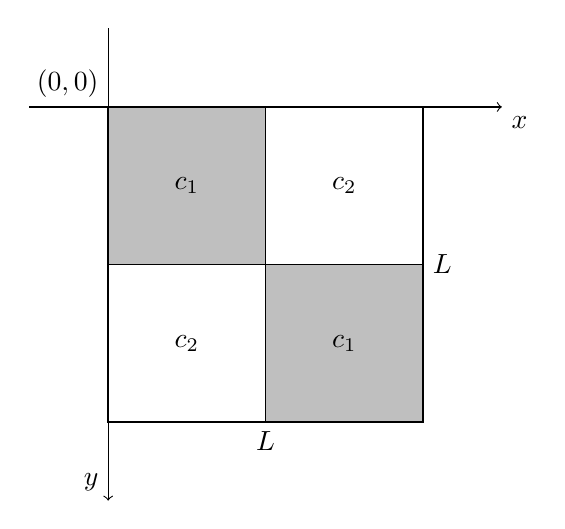
\begin{tikzpicture}[scale=2.0]
        \draw[fill=white] (0,0) rectangle (1,1);
        \draw[fill=white] (1,1) rectangle (2,2);
        \draw[fill=gray!50] (0,1) rectangle (1,2);
        \draw[fill=gray!50] (1,0) rectangle (2,1);
        
        % Draw the boundary of the square
        \draw[thick] (0,0) rectangle (2,2);
    
        % Draw axes
        \draw[->] (-0.5,2) -- (2.5,2) node[anchor=north west] {$x$};  % x-axis
        \draw[<-] (0,-0.5) node[anchor=south east] {$y$} -- (0,2.5);  % y-axis
    
        % Mark the origin
        \node[anchor=south east] at (0,2) {$(0, 0)$};
        
        % Mark the side length L
        \draw[-] (2,0) -- (2,2) node[midway, right] {$L$};
        \draw[-] (0,0) -- (2,0) node[midway, below] {$L$};
        \draw (0.5, 1.5) node[anchor=center] {$c_1$};
        \draw (1.5, 0.5) node[anchor=center] {$c_1$};
        \draw (1.5, 1.5) node[anchor=center] {$c_2$};
        \draw (0.5, 0.5) node[anchor=center] {$c_2$};
    \end{tikzpicture}
    \caption{Dvimačio modelio pradinės sąlygos laiku $t=0$. Pilka spalva žymi plotą priklausantį aibei $A$. }
\end{figure}

\section{Skaitinis modelis}

\subsection{Erdvės diskretizavimas Dekarto koordinačių sistemoje}

Dviejų dimensijų skaitiniam modeliui erdvė buvo padalinta į $N \times M$ taškų 
nutolusių vienas nuo kito fiksuotais $\Delta x$ ir $\Delta y$ atstumais.

\begin{figure}[!h]
\centering
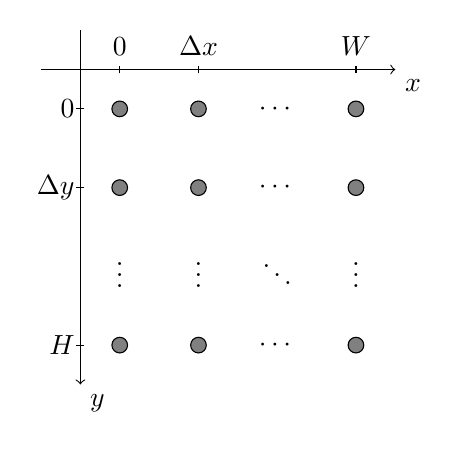
\begin{tikzpicture}

   % Set up styles for the grid
  \tikzset{
    node/.style={circle, draw, fill=gray, inner sep=2pt},
    ellipsis/.style={draw=none, fill=none}
  }

  \draw[->] (0, -0.5) -- (4.5, -0.5) node[anchor=north west] {$x$};  % x-axis
  % x-axis ticks
  \draw[-] (1, -0.55) -- (1, -0.45) node[anchor=south] {$0$};
  \draw[-] (2, -0.55) -- (2, -0.45) node[anchor=south] {$\Delta x$};
  \draw[-] (4, -0.55) -- (4, -0.45) node[anchor=south] {$W$};
  
  \draw[<-] (0.5,-4.5) node[anchor=north west] {$y$} -- (0.5, 0);  % y-axis
  % y-axis ticks
  \draw[-] (0.45, -1) -- (0.55, -1) node[anchor=east] {$0$};
  \draw[-] (0.45, -2) -- (0.55, -2) node[anchor=east] {$\Delta y$};
  \draw[-] (0.45, -4) -- (0.55, -4) node[anchor=east] {$H$};


  % Draw the 3x3 grid of colored circles in a 4x4 layout
  \foreach \x in {1, 2, 4} {
    \foreach \y in {1, 2, 4} {
      \node[node] at (\x, -\y) {};
    }
  }

  % Add ellipses in the 4th row and column for continuation

  \node[ellipsis] at (3, -1) {$\cdots$};
  \node[ellipsis] at (3, -2) {$\cdots$};
  \node[ellipsis] at (3, -4) {$\cdots$};

  \node[ellipsis] at (1, -3) {$\vdots$};
  \node[ellipsis] at (2, -3) {$\vdots$};
  \node[ellipsis] at (4, -3) {$\vdots$};

  \node[ellipsis] at (3, -3) {$\ddots$};

\end{tikzpicture}
\caption{ diskretizuota erdvė }
\end{figure}

Čia 

\newpage
\subsection{Dviejų dimensijų skaitinis modelis Dekarto koordinačių sistemoje}

Remiantis išreikštiniu baigtinių skirtumų metodu iš dvimačio modelio galima gauti skaitinį modelį.
\begin{subequations} \label{numerical-eqs}
\begin{align}
\frac{c^{n+1}_{1,i,j}-c^n_{1,i,j}}{\Delta t}&=
-3c^{n}_{1,i,j}c^{n}_{2,i,j}\notag\\
&+D\left(\frac{c^n_{1,i-1,j}-2c^n_{1,i,j}+c^n_{1,i+1,j}}{(\Delta x)^2}+\frac{c^n_{1,i,j-1}-2c^n_{1,i,j}+c^n_{1,i,j+1}}{(\Delta y)^2}\right)\\
\frac{c^{n+1}_{2,i,j}-c^n_{2,i,j}}{\Delta t}&=
-5c^{n}_{1,i,j}c^{n}_{2,i,j}\notag\\
&+D\left(\frac{c^n_{2,i-1,j}-2c^n_{2,i,j}+c^n_{2,i+1,j}}{(\Delta x)^2}+\frac{c^n_{2,i,j-1}-2c^n_{2,i,j}+c^n_{2,i,j+1}}{(\Delta y)^2}\right)\\
\frac{c^{n+1}_{3,i,j}-c^n_{3,i,j}}{\Delta t}&=2c^{n}_{1,i,j}c^{n}_{2,i,j},
\end{align}
\end{subequations}

kur $n\in[0, T)$ - laiko momentas, 
$i\in[0,N)$ - diskrečios erdvės taško koordinatė $x$ ašyje,
$j\in[0,M)$ - diskrečios erdvės taško koordinatė $y$ ašyje,
$c^n_{1,i,j}$ - pirmos medžiagos kiekis diskrečios erdvės taške $i$, $j$ laiko momentu $n$,
$c^n_{2,i,j}$ - antros medžiagos kiekis diskrečios erdvės taške $i$, $j$ laiko momentu $n$,
$c^n_{3,i,j}$ - trečios medžiagos kiekis diskrečios erdvės taške $i$, $j$ laiko momentu $n$,
$\Delta t$ - laiko žingsnis,
$\Delta x$ - diskrečios erdvės žingsnis $x$ ašimi,
$\Delta y$ - diskrečios erdvės žingsnis $y$ ašimi.

\subsection{Modelio skaitinis stabilumas}

Norint užtikrinti skaitinį programos stabilumą, reikia užtikrinti, kad visais laiko momentais, visuose diskretizuotos erdvės taškuose, visų medžiagų koncentracijos išliktų ne neigiamos. Parodysime, kad tai užtikrinti, užtenka pasirinkti pakankamai mažą laiko žingsnį $\Delta t$. Pirmiausia įvedame porą konstantų:
\begin{align*}
\mu_x = \frac{D\Delta t}{(\Delta x)^2}, \quad
\mu_y = \frac{D\Delta t}{(\Delta y)^2}
\end{align*}

Tada pertvarkome dviejų dimensijų skaitinį modelį \eqref{numerical-eqs} taip, kad kairėsė lygčių pusėse liktų medžiagų koncentracija laiko momentu $n+1$, o dešinėse lygčių pusėse sugrupuojame narius pagal medžiagų koncentracija skirtinguose diskretizuotos erdvės taškuose:

\begin{subequations} \label{eqs:r-coefs}
    \begin{align}
    c^{n+1}_{1,i,j}&=\underbrace{(1-3\Delta tc^{n}_{2,i,j}-2(\mu_x+\mu_y))}_{R_1}c^n_{1,i,j}+\mu_xc^n_{1,i-1,j}+\mu_xc^n_{1,i+1,j}+\mu_yc^n_{1,i,j-1}+\mu_yc^n_{1,i,j+1} \label{r-coefs1}\\
    c^{n+1}_{2,i,j}&=\underbrace{(1-5\Delta tc^{n}_{1,i,j}-2(\mu_x+\mu_y))}_{R_2}c^n_{2,i,j}+\mu_xc^n_{2,i-1,j}+\mu_xc^n_{2,i+1,j}+\mu_yc^n_{2,i,j-1}+\mu_yc^n_{2,i,j+1} \label{r-coefs2}\\
    c^{n+1}_{3,i,j}&=c^n_{3,i,j}+2\Delta tc^{n}_{1,i,j}c^{n}_{2,i,j} \label{r-coefs3}
    \end{align}
\end{subequations}

% \begin{subequations} \label{mu-eqs}
%     \begin{align}
%     c^{n+1}_{1,i,j}&=c^n_{1,i,j}-3\Delta tc^{n}_{1,i,j} c^{n}_{2,i,j}+\mu_x(c^n_{1,i-1,j}-2c^n_{1,i,j}+c^n_{1,i+1,j})+\mu_y(c^n_{1,i,j-1}-2c^n_{1,i,j}+c^n_{1,i,j+1})\\
%     c^{n+1}_{2,i,j}&=c^n_{2,i,j}-5\Delta tc^{n}_{1,i,j} c^{n}_{2,i,j}+\mu_x(c^n_{2,i-1,j}-2c^n_{2,i,j}+c^n_{2,i+1,j})+\mu_y(c^n_{2,i,j-1}-2c^n_{2,i,j}+c^n_{2,i,j+1})\\
%     c^{n+1}_{3,i,j}&=c^n_{3,i,j}+2\Delta tc^{n}_{1,i,j}c^{n}_{2,i,j}
%     \end{align}
% \end{subequations}

Baziniu atveju, kai $n=0$, medžiagų koncentracija visuose taškuose yra ne neigiama, kaip numatyta pradinėje sąlygoje \eqref{intial-cond}. Darome indukcijos hipotezės prielaidą, kad medžiagų koncentracija visuose diskretizuotos erdvės taškuose, laiko momentu $n$ bus ne neigiama:

\begin{align} \label{induction-assumption}
    c^n_{k,i,j} \geqslant 0, \quad k=1,2,3,\quad i=0,1,\dots,N-1,\quad j=0,1,\dots,M-1
\end{align}

Akivaizdu, kad lygtyje \eqref{r-coefs3}, medžiagos koncentracija $c^{n+1}_{3,i,j}$ negali tapti neigiama dėl prielaidos \eqref{induction-assumption} ir fakto, kad $\Delta t>0$. Pirmos medžiagos lygtyje \eqref{r-coefs1}, galima pastebėti, kad dėmenys su medžiagų koncentracijomis iš aplinkinių diskretizuotos erdvės taškų visada bus ne neigiami dėl prielaidos \eqref{induction-assumption} ir fakto, kad $\mu_x>0$ ir $\mu_y>0$:

\begin{align*}
    \mu_xc^n_{1,i-1,j}+\mu_xc^n_{1,i+1,j}+\mu_yc^n_{1,i,j-1}+\mu_yc^n_{1,i,j+1}\geqslant 0
\end{align*}

Taigi $c^{n+1}_{1,i,j}$ ženklą lemia tik koeficientas $R_1$, todėl įvedame ribojimą, kad $R_1\geqslant 0$. Analogiškai, iš antros medžiagos lygties \eqref{r-coefs2} gauname, kad $R_2\geqslant 0$ ir turime neligybių sistemą:

\begin{align}
  \begin{cases}
    (1-3\Delta tc^{n}_{2,i,j}-2(\mu_x+\mu_y))\geqslant 0\\
    (1-5\Delta tc^{n}_{1,i,j}-2(\mu_x+\mu_y))\geqslant 0
  \end{cases}, \quad i=0,1,\dots,N-1, \quad j=0,1,\dots,M-1
\end{align}

Pertvarke neligybes gauname:

\begin{align}
  \begin{cases}
    \Delta t \leqslant (3c^{n}_{2,i,j}+2D((\Delta x)^{-2}+(\Delta y)^{-2}))^{-1}\\
    \Delta t \leqslant (5c^{n}_{1,i,j}+2D((\Delta x)^{-2}+(\Delta y)^{-2}))^{-1}
  \end{cases}
\end{align}

% \begin{cases}
%     1-\Delta t\left(3c^{n}_{2,i,j}+2D\left(\frac{1}{(\Delta x)^2}+\frac{1}{(\Delta y)^2}\right)\right)\geq 0\implies
%     \Delta t\leq\frac{1}{3c^{n}_{2,i,j}+2D\left((\Delta x)^{-2}+(\Delta y)^{-2}\right)}\\
%     1-\Delta t\left(5c^{n}_{1,i,j}+2D\left(\frac{1}{(\Delta x)^2}+\frac{1}{(\Delta y)^2}\right)\right)\geq 0\implies
%     \Delta t\leq\frac{1}{5c^{n}_{1,i,j}+2D\left((\Delta x)^{-2}+(\Delta y)^{-2}\right)}
% \end{cases}

\newpage
Galima panaikinti laiko žingsnio $\Delta t$ priklausomybę nuo einamojo diskrečios erdvės taško padarius pastebėjimą,
kad laiko žingsnis su didžiausiomis medžiagų kiekių $c^n_{1,i,j}$ bei $c^n_{2,i,j}$ reikšmėmis užtikrintų stabilumą visiem
likusiems diskrečios erdvės taškams, taigi:

\begin{align*}
    \Delta t\leq\min\left(
    \frac{1}{3\max\limits_{(i,j,n)\in[0,N)\times[0,M)\times[0,T)}c^{n}_{2,i,j}
    +2D\left((\Delta x)^{-2}+(\Delta y)^{-2}\right)},\right.\\
    \left. \frac{1}{5\max\limits_{(i,j,n)\in[0,N)\times[0,M)\times[0,T)}c^{n}_{1,i,j}
    +2D\left((\Delta x)^{-2}+(\Delta y)^{-2}\right)}
    \right)
\end{align*}

Taip pat galime atsikratyti laiko žingsnio $\Delta t$ priklausomybės nuo einamojo laiko momento, nes
pagal duotas kraštines sąlygas į sistemą laikui einant nepatenka joks naujas medžiagų $c_1$ ir $c_2$ kiekis.
Taip pat vykstant medžiagų $c_1$ ir $c_2$ reakcijai, bendri šių medžiagų kiekiai uždaroje sistemoje mažės, todėl:

\begin{align*}
    \Delta t\leq\min\left(
        \frac{1}{3\max\limits_{(i,j)\in[0,N)\times[0,M)}c^{0}_{2,i,j}
        +2D\left((\Delta x)^{-2}+(\Delta y)^{-2}\right)},\right. \\
        \left. \frac{1}{5\max\limits_{(i,j)\in[0,N)\times[0,M)}c^{0}_{1,i,j}
        +2D\left((\Delta x)^{-2}+(\Delta y)^{-2}\right)}
    \right)
\end{align*}

Šiuo atveju, iš pradinių sąlygų $\max\limits_{(i,j)\in[0,N)\times[0,M)}c^{0}_{2,i,j}=\max\limits_{(i,j)\in[0,N)\times[0,M)}c^{0}_{1,i,j}=1$, taigi

\begin{align*}
    \Delta t\leq\frac{1}{5+2D\left((\Delta x)^{-2}+(\Delta y)^{-2}\right)}
\end{align*}
\section{Programos sudarymas ir rezultatai}

Pagal dviejų dimensijų skaitinį modelį \eqref{numerical-eqs} sudarytas uždavinį sprendžiantis skriptas ir kiti pagalbiniai skriptai duomenims vaizduoti ir tikrinti. Skriptai rašomi \textit{Python} programavimo kalba, naudojant \textit{NumPy}, \textit{SciPy}, \textit{Matplotlib} paketus. 

Modelio rezultatai yra saugomi kaip atskiri \textit{.npy} formato failai, kurie yra skirti saugoti \mbox{\textit{NumPy}} masyvus. Dėl praktinių rezultatų panaudojimo ir tyrimo nebūtina saugoti informacijos apie visus laiko žingsnius, todėl išsaugotuose rezultatų failuose, simuliacijos kadrai laiko kryptimi gali būti praretinti iki tūkstančio kartų, priklausomai nuo pasirinktų parametrų. Pagalbiniai duomenų vaizdavimo skriptai šiuos duomenis agreguoja į grafikus, kurie išsaugomi \textit{.png} formatu.


\begin{figure}[h!]
\centering
\includegraphics[width=\textwidth]{../assets/examples-c1.png} \\
\includegraphics[width=\textwidth]{../assets/examples-c2.png} \\
\includegraphics[width=\textwidth]{../assets/examples-c3.png}
\caption{Kompiuterinio modelio rezultato pavyzdys. $D = 0.05$, $W = 1$, $H = 1$, $\Delta x = \frac{1}{99}$, $\Delta y = \frac{1}{99}$, $k = 1$, $c_0 = 1$, $\Delta t$ - pasirinktas pagal \eqref{numerical-stability-condition} }
%     \label{result-example}
\end{figure}

\subsection{Rezultatų korektiškumo tikrinimas}

% Čia galima tikrint kad individualiu ląstelių
% - keičiant dx/dy kiekio per laiką sprendinys vizualiai konverguoja
% - kiekio grafikai per laika medžiagom c1 ir c2 mažėja, o c3 - didėja.
% - jei nustatom reakcijos koeficienta k = 0, kiekis bus pastovus
Tikrinti rezultatų korektiškumui yra naudojami tie patys duomenys kaip ir rezultatų vaizdavimui. Pirmiausia galime patikrinti kaip šio modelio sprendinys keičiasi didinant erdvinius žingsnius $\Delta x$ ir $\Delta y$.




\subsection{Palyginimas su eksperimentiniais duomenimis}


\section{Maišymo modeliavimas}

\subsection{Reakcijos stabdymo sąlyga}

Kompiuterinio modelio rezultatai rodo, kad vykstant reakcijai, reagentų kiekis erdvėje artėja prie 0, tačiau niekad jo nepasiekia. Tai būdinga ir realybėje vykstančioms reakcijoms, dėl šios priežasties kompiuterinio modelio darbą stabdysime, kai sureaguos $\eta_\text{stop}\%$ pradinių medžiagų kiekio. Matematiškai reakcijos stabdymo laiką $t_\text{stop}$ galime apibrėžti taip:

\begin{align}
    q(t_\text{stop})=\left(1-\frac{\eta_\text{stop}}{100}\right)q(0),\quad \eta_\text{stop}\in[0, 100)
\end{align}

Tolimesniems pavyzdžiams ir analizei naudosime konkrečią reikšmę $\eta_\text{stop}=97$ ir reakciją stabdysime laiku $t_\text{stop}$, kai $q(t_\text{stop})=0.03q(0)$. Toks procentas pasirinktas todėl, kad sureagavus 97\% reagentų, reakcija iš esmės yra pasibaigusi ir gautų duomenų užtenka atlikti analizei.

\subsection{Atsitiktinis maišymas}

Konstruojant kompiuterinį modelį šiam procesui atkreipsime dėmesį į kelias svarbias detales:

\begin{itemize}
  \item Išmaišymas vyksta prie daug žemesnės temperatūros negu reakcija
  \item Išmaišymas gali vykti kelis kartus
  \item Išmaišymo procesas nėra deterministinis
\end{itemize}

\paragraph{Maišymas prie žemesnės temperatūros}

Kadangi maišymas vyksta prie daug žemesnės temperatūros negu pati reakcija, darysime prielaidą, kad ištraukus reagentus iš krosnies cheminė reakcija ir difuzija nevyksta, todėl medžiagų maišymą modeliuosime kaip momentinį procesą, kuris įvyksta tarp diskrečių laiko žingsnių.

\paragraph{Maišymas kelis kartus}

Praktikoje vykdant šią reakcija chemikai savo nuožiūra pasirenka laiką, kuriuo vykdys išmaišymą, todėl ir kompiuterinis modelis turėtų suteikti vartotojui pasirinkimą nurodyti konkrečius laiko momentus, kada vyks medžiagų išmaišymas. Šiuos laikus žymėsime taip:

\begin{align}
    t^1_\text{mix}, t^2_\text{mix}, \dots, t^{T^*}_\text{mix} \quad T^*\in \mathbb{N}
\end{align}

Čia $T^*$ -- bendras išmaišymų skaičius, o $t^i_\text{mix}$ -- $i$-tojo išmaišymo laikas. Kadangi kompiuterinis modelis laiko informaciją apie diskrečius laiko taškus $t_n$, mes negalime tiesiogiai apibrėžti sąlygos, kad išmaišymas vyks konkrečiu laiko momentu $t^i_\text{mix}$, todėl medžiagas išmaišysime einamajame laiko žingsnyje $t_n$, kuris yra artimiausias išmaišymo laikui $t^i_\text{mix}$:

\newpage

\begin{figure}[!h]
\centering
\label{mix-inequality-graphic}
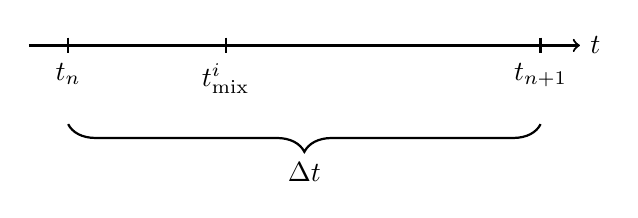
\begin{tikzpicture}[thick]

% Main timeline
\draw[->] (-0.5,0) -- (6.5,0) node[right] {$t$}; % Timeline with axis label

% Time points
\foreach \x/\label in {0/{$t_n$}, 2/{$t^i_\text{mix}$}, 6/{$t_{n+1}$}} {
    \draw (\x,0.1) -- (\x,-0.1) node[below] {\label};
}

% Braces for interval
\draw[decorate,decoration={brace,amplitude=10pt,mirror}] (0,-1) -- (6,-1) node[midway,below=10pt] {$\Delta t$};


\end{tikzpicture}
\caption{Šiuo atveju, išmaišymas įvyks laiko žingsniu $t_n$, o ne $t_{n+1}$, nes $t^i_\text{mix}$ yra arčiau laiko momento $t_n$}
\end{figure}

arba kitaip sakant išmaišymas įvyks laiko žingsniu $t_n$, jei:

\begin{align}
    \vert t_n - t^i_\text{mix} \vert < \frac{1}{2}\Delta t \label{mix-inequality}
\end{align}

\paragraph{Nedeterministinis maišymas}

Maišymas praktikoje yra chaotiškas procesas, todėl sudarydami kompiuterinį modelį turime į tai atsižvelgti. Maišymą modeliuosime kaip reakcijos erdvės sričių atsitiktinį išdėstymą. Pradinė erdvę $\Omega$ padalinsime į mažesnes, nepersidengiančias, vienodas kvadratines sritis $\Omega_i$, tada sugeneruosime atsitiktinę $4$-permutaciją $\sigma$ ir $4$ atsitiktinius kampus $\theta_i \in \{0, \frac{\pi}{2}, \pi, \frac{3\pi}{2}\}$. Kiekviena iš sričių $\Omega_i$ keliauja į poziciją, kurioje yra sritis $\Omega_{\sigma(i)}$, tačiau pasukta kampu $\theta_i$. 

\begin{figure}[!h]
\centering
\label{split-reaction-space}

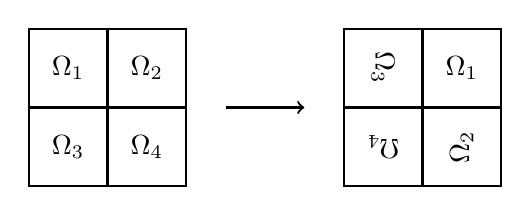
\begin{tikzpicture}
    % Original Grid
    \draw[thick] (0,0) rectangle (2,2);
    \draw[thick] (1,0) -- (1,2);
    \draw[thick] (0,1) -- (2,1);

    \node at (0.5,1.5) {$\Omega_1$};
    \node at (1.5,1.5) {$\Omega_2$};
    \node at (0.5,0.5) {$\Omega_3$};
    \node at (1.5,0.5) {$\Omega_4$};

    % Arrow
    \draw[->, thick] (2.5,1) -- (3.5,1);

    % Transformed Grid
    \begin{scope}[shift={(4,0)}]
        \draw[thick] (0,0) rectangle (2,2);
        \draw[thick] (1,0) -- (1,2);
        \draw[thick] (0,1) -- (2,1);

        \node at (0.5,1.5) {\rotatebox{270}{$\Omega_3$}}; % Rotated 180° horizontally
        \node at (1.5,1.5) {$\Omega_1$};             % No change
        \node at (0.5,0.5) {\rotatebox{180}{$\Omega_4$}}; % Upside down
        \node at (1.5,0.5) {\rotatebox{90}{$\Omega_2$}};  % 90° rotation
    \end{scope}
\end{tikzpicture}
\caption{Maišymo transformacijos pavyzdys}
\end{figure}

\newpage
\subsection{Atsitiktinio maišymo rezultatai}

% \begin{figure}[h!]
% \centering
% \includegraphics[width=\textwidth]{assets/rnd-mix-c0-1.png} \\
% \includegraphics[width=\textwidth]{assets/rnd-mix-c1-1.png} \\
% \includegraphics[width=\textwidth]{assets/rnd-mix-c2-1.png}

% \caption{Kompiuterinio modelio rezultatai - medžiagų koncentracijos per laiką, kai vyksta išmaišymas. Išmaišymo laikas $t^1_\text{mix} = 1h\,30min$ }

% \label{mix-example}
% \end{figure}

\begin{figure}[h]
    \centering
    \begin{minipage}[c]{0.40\textwidth}
        \centering
        \includegraphics[width=\textwidth]{assets/rnd-mix-left-c0-1.png}\\
        \includegraphics[width=\textwidth]{assets/rnd-mix-left-c1-1.png}\\
        \includegraphics[width=\textwidth]{assets/rnd-mix-left-c2-1.png}
    \end{minipage}%
    \hfill
    \begin{minipage}[c]{0.1\textwidth}
        \centering
        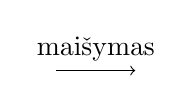
\begin{tikzpicture}
            \draw[->] (0,0.5) -- (1,0.5);
            \node[above] at (0.5, 0.5) {maišymas};
        \end{tikzpicture}
    \end{minipage}%
    \hfill
    \begin{minipage}[c]{0.45\textwidth}
        \centering
        \includegraphics[width=\textwidth]{assets/rnd-mix-right-c0-1.png}\\
        \includegraphics[width=\textwidth]{assets/rnd-mix-right-c1-1.png}\\
        \includegraphics[width=\textwidth]{assets/rnd-mix-right-c2-1.png}
    \end{minipage}

    \caption{Kompiuterinio modelio rezultatai - medžiagų koncentracijos per laiką, kai vyksta išmaišymas. Išmaišymo laikas $t^1_\text{mix} = 1h\,30min$ }

    \label{mix-example}

\end{figure}

\ref{mix-example}-ame pavyzdyje matome kaip atrodo reakcijos eiga, kada vyksta išmaišymas. Trečiame stulpelyje ir ypatingai trečios medžiagos koncentracijoje matome ryškių artefaktų. Taip yra todėl, kad nuo išmaišymo praejo labai mažai laiko ir medžiagos nespėjo sureaguoti naujoje aplinkoje. Tarp laiko momentų $t=1h\,30min$ ir $t=5h\,59min$ trečios medžiagos $c_3$ koncentracija daugiausiai keitėsi tose vietose, kuriose iš pradžių vyko reakcija, tačiau galime matyti ir visiškai naujos sienelės susidaryma ties srities viduriu. Norint geriau suprasti kokį poveikį toks išmaišymas turi reakcijos pabaigos lakui reikėtų ištirti trečios medžiagos koncentracijos priklausomybę nuo laiko.

\newpage
\begin{figure}[h!]
    \centering
    \includegraphics[width=0.5\textwidth]{assets/bad-mix-qnt-1.png}
    \caption{Kompiuterinio modelio rezultatų palyginimas, kai išmaišymas vyksta ir nevyksta.  }
    \label{bad-mix-qnt-example}
\end{figure}
\ref{bad-mix-qnt-example}-ame pavyzdyje puikiai matosi, kad išmaišymas nepagreitino reakcijos, o ją sulėtino. Reakcijos laikas su išmaišymu yra apytiksliai dvejom su puse valandom ilgesnis. Ši problema atsiranda todėl, kad mes modeliuojame ypač mažą reakcijos erdvės sritį, kurioje susiduria tik 4 mikrodalelės, dėl to nėra daug skirtingų išdėstymų, kada viena sienele galėtų dalintis skirtingų medžiagų dalelės, prie to žinoma prisideda ir faktas, kad šis modelis yra dviejų dimensijų. Eksperimentas parodė, kad nesuveiktų ir statistinis bandymas - vidutinis atsitiktinis išmaišymas taip pat neduoda geresnių rezultatų negu reakcijos modelis be išmaišymų. Dėl šios priežasties apsvarstysime alternatyvų išmaišymo metoda.

\subsection{Tobulas maišymas}

Kad išspręstume atsitiktinio maišymo problemą, modeliuosime tobulą teorinį išmaišymą, kuris turės didžiausią poveikį reakcijos greičiui. Pats maišymo modelis išliks toks pat, tačiau sritis $\Omega_i$ sudėliosime ne atsitiktinai, o sukeisime įstrižai. Tobulas išmaišymas aišku priklauso nuo pradinių sąlygų, o šis galioja tik duotoms pradinėms sąlygoms \eqref{intial-cond}.

\begin{figure}[!h]
\centering
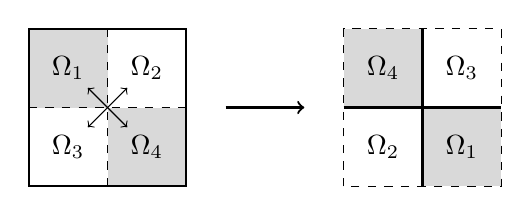
\begin{tikzpicture}
    % Original Grid
    \fill[gray!30] (0,1) rectangle (1, 2);
    \fill[gray!30] (1,0) rectangle (2, 1);
    \draw[<->] (0.75,0.75) -- (1.25,1.25);
    \draw[<->] (1.25,0.75) -- (0.75,1.25);
    \draw[thick] (0,0) rectangle (2,2);
    \draw[dashed] (1,0) -- (1,2);
    \draw[dashed] (0,1) -- (2,1);

    \node at (0.5,1.5) {$\Omega_1$};
    \node at (1.5,1.5) {$\Omega_2$};
    \node at (0.5,0.5) {$\Omega_3$};
    \node at (1.5,0.5) {$\Omega_4$};

    % Arrow
    \draw[->, thick] (2.5,1) -- (3.5,1);

    % Transformed Grid
    \begin{scope}[shift={(4,0)}]
        \fill[gray!30] (0,1) rectangle (1, 2);
        \fill[gray!30] (1,0) rectangle (2, 1);
        
        \draw[dashed] (0,0) rectangle (2,2);
        \draw[thick] (1,0) -- (1,2);
        \draw[thick] (0,1) -- (2,1);

        \node at (0.5,1.5) {$\Omega_4$};
        \node at (1.5,1.5) {$\Omega_3$};
        \node at (0.5,0.5) {$\Omega_2$};
        \node at (1.5,0.5) {$\Omega_1$};
    \end{scope}
\end{tikzpicture}
\caption{Tobulo maišymo transformacija}
\label{perfect-2x2-mix}
\end{figure}
\ref{perfect-2x2-mix}-ame pavyzdyje matoma prieš tai apibūdintą transformacija. Punktyrinės linijos kairėje pusėje žymi sieneles ties kuriomis vyksta reakcija. Šiuo atveju po išmaišymo nėra sričių, kurios turėtų bendrą punktyrinę sienelę, o tai reiškia, kad tokiu būdu sumaišius sritis, visos vidinės sienelės turės didžiausią įmanomą skirtingų medžiagų kontrastą, kuris lems didžiausią įmanomą reakcijos pagreitėjimą.
\newpage
\begin{figure}[h!]
    \centering
    \includegraphics[width=0.5\textwidth]{../paper/assets/optimal-mix-qnt-1.png}

    \caption{Kompiuterinio modelio rezultatų palyginimas tarp reakcijos be išmaišymo ir reakcijos su tobulu išmaišymu.  }

    \label{optimal-mix-qnt}
\end{figure}

Šiuo atveju, \ref{optimal-mix-qnt}-ame pavyzdyje matome, kad dėl tobulo išmaišymo galime matyti šuolį medžiagos kiekyje. Toks maišymas turi teigiamą poveikį reakcijos pabaigos laikui ir labiau atitinka eksperimentinius rezultatus negu atsitiktinis išmaišymas.
Čia galime pasamprotauti, kaip reakcijos pabaigos laikas priklauso nuo išmaišymo laiko - jei išmaišome pradinę konfigūraciją pačioje reakcijos pradžioje, rezultatams tai neturės jokios įtakos ir gausime reakcijos modelį be išmaišymo. Lygiai tas pats nutiktų jei išmaišymas įvyktų ką tik prieš reakcijos pabaigą, tačiau išmaišymas kitais laiko momentais, kaip jau matėme, gali sutrumpinti reakcijos pabaigos laiką. Jei pavaizduotume reakcijos pabaigos laiko priklausomybę nuo išmaišymo laiko, gautume štai tokį grafiką:

\begin{figure}[h!]
    \centering
    \includegraphics[width=0.5\textwidth]{../paper/assets/mix-end-1.png}

    \caption{Kompiuterinio modelio rezultatai - reakcijos pabaigos laiko priklausomybė nuo išmaišymo laiko. }

    \label{mix-end}
\end{figure}

\ref{mix-end}-ame pavyzdyje matome, kad priklausomybė nėra simetriška, reakcijos pabaigos laikas, kai išmaišymas nevyksta, yra $11h\, 30min$. Optimalus išmaišymo laikas yra $1h\, 30min$ ir tokiu atveju 97\% medžiagų sureaguos per $9h\,33min$.

\subsection{Maišymo modeliavimas didesnėje erdvėje}

Modeliuoti mažą visos reakcijos erdvės sritį užtenka norint gauti tikslias aproksimacijas difuzijos bei reakcijos greičio konstantoms \cite{mackeviciusCloserLookComputer2012}. Tačiau modeliuodami medžiagų išmaišymą neturime priežasties daryti tokios pačios prielaidos. Norint modeliuoti didesnę erdvę, pradines sąlygas reikia atkartoti veidrodiniu principu, tuo galima įsitikinti pažvelgus į \ref{fig:periodic-space}-ą pavyzdį. Modeliuodami didesnę erdvę, ne tik padidės srities plotas, kaip pavaizduota \ref{large-initial-conditions}-ame pavyzdyje, tačiau ir padvigubinsime diskrečių taškų kiekį kiekviena erdvine kryptimi.


\begin{figure}[h!]
\centering
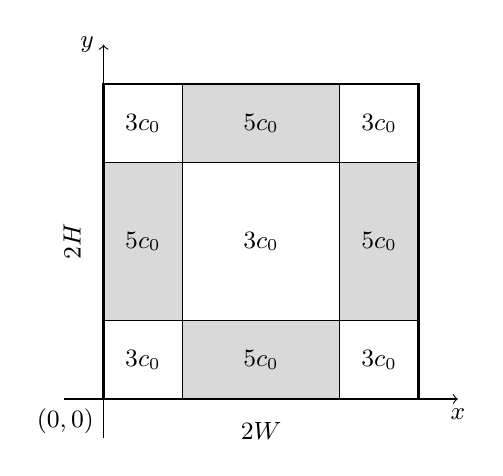
\begin{tikzpicture}
  
    % Fill the boundary cells
    % \fill[gray!30] (0, 3) rectangle (1, 4); % Top-left
    \fill[gray!30] (1, 3) rectangle (3, 4); % Top
    % \fill[gray!30] (3, 3) rectangle (4, 4); % Top-right
    \fill[gray!30] (0, 1) rectangle (1, 3); % Left
    \fill[gray!30] (3, 1) rectangle (4, 3); % Right
    % \fill[gray!30] (0, 0) rectangle (1, 1); % Bottom-left
    \fill[gray!30] (1, 0) rectangle (3, 1); % Bottom
    % \fill[gray!30] (3, 0) rectangle (4, 1); % Bottom-right

    % Draw the outer rectangle
    \draw[thick] (0, 0) rectangle (4, 4);
    \node at (2, -0.4) {\small $2W$};
    \node[rotate=90] at (-0.4, 2) {\small $2H$};

    % Draw the inner rectangle
    \draw[-] (0, 1) -- (4, 1);
    \draw[-] (0, 3) -- (4, 3);
    \draw[-] (1, 0) -- (1, 4);
    \draw[-] (3, 0) -- (3, 4);

    % Labels
    \node at (0.5, 3.5) {\small $3c_0$};
    \node at (2, 3.5) {\small $5c_0$};
    \node at (3.5, 3.5) {\small $3c_0$};

    \node at (0.5, 2) {\small $5c_0$};
    \node at (2, 2) {\small $3c_0$};
    \node at (3.5, 2) {\small $5c_0$};

    \node at (0.5, 0.5) {\small $3c_0$};
    \node at (2, 0.5) {\small $5c_0$};
    \node at (3.5, 0.5) {\small $3c_0$};

    % Coordinate axes
    \draw[->] (-0.5, 0) -- (4.5, 0) node[anchor=north] {\small $x$};
    \draw[->] (0, -0.5) -- (0, 4.5) node[anchor=east] {\small $y$};
    \node[anchor=north east] at (0, 0) {\small $(0,0)$};
\end{tikzpicture}
\caption{ Praplėstos pradinės sąlygos. }

\label{large-initial-conditions}
\end{figure}

Kadangi prieš tai apibrėžtas maišymo modelis yra tinkamas tik įprastoms pradinėms \hbox{sąlygoms \eqref{intial-cond}}, praplėstoms pradinėms sąlygoms reikės atskirai apibrėžti išmaišymą. Eksperimentas parodė, kad net su praplėstomis pradinėmis sąlygomis, atsitiktinio maišymo problema nedingsta - išmaišymas dažniausiai pailgina reakcijos pabaigos laiką. Dėl šios priežasties praplėsime tobulo išmaišymo modelį analogiškai atkartodami jį veidrodžio principu kaip ir pradines sąlygas. 

\begin{figure}[!h]
\centering
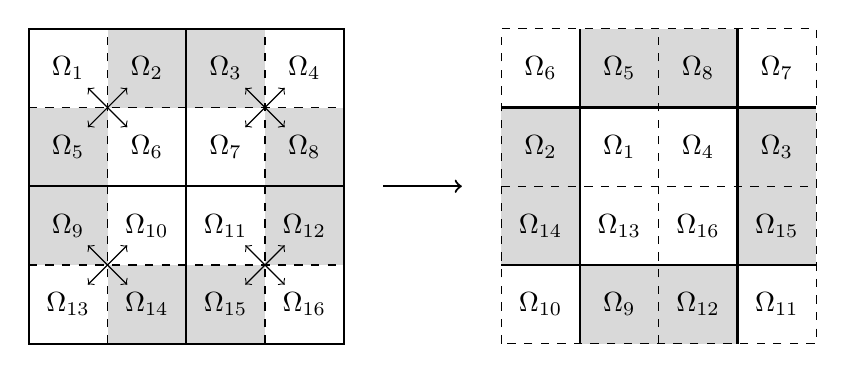
\begin{tikzpicture}
    % Original Grid

    \fill[gray!30] (1, 0) rectangle (3, 1);
    \fill[gray!30] (1, 3) rectangle (3, 4);

    \fill[gray!30] (0, 1) rectangle (1, 3);
    \fill[gray!30] (3, 1) rectangle (4, 3);

    \draw[thick] (0,0) rectangle (2,2);
    \draw[thick] (0,2) rectangle (2,4);
    \draw[thick] (2,0) rectangle (4,2);
    \draw[thick] (2,2) rectangle (4,4);
    \draw[dashed] (1,0) -- (1,4);
    \draw[dashed] (0,1) -- (4,1);
    \draw[dashed] (3,0) -- (3,4);
    \draw[dashed] (0,3) -- (4,3);

    \draw[<->] (0.75,0.75) -- (1.25,1.25);
    \draw[<->] (1.25,0.75) -- (0.75,1.25);

    \draw[<->] (2.75,0.75) -- (3.25,1.25);
    \draw[<->] (3.25,0.75) -- (2.75,1.25);

    \draw[<->] (0.75,2.75) -- (1.25,3.25);
    \draw[<->] (1.25,2.75) -- (0.75,3.25);

    \draw[<->] (2.75,2.75) -- (3.25,3.25);
    \draw[<->] (3.25,2.75) -- (2.75,3.25);

    \node at (0.5,3.5) {$\Omega_1$};
    \node at (1.5,3.5) {$\Omega_2$};
    \node at (0.5,2.5) {$\Omega_5$};
    \node at (1.5,2.5) {$\Omega_6$};

    \node at (2.5,3.5) {$\Omega_3$};
    \node at (3.5,3.5) {$\Omega_4$};
    \node at (2.5,2.5) {$\Omega_7$};
    \node at (3.5,2.5) {$\Omega_8$};

    \node at (0.5,1.5) {$\Omega_9$};
    \node at (1.5,1.5) {$\Omega_{10}$};
    \node at (0.5,0.5) {$\Omega_{13}$};
    \node at (1.5,0.5) {$\Omega_{14}$};

    \node at (2.5,1.5) {$\Omega_{11}$};
    \node at (3.5,1.5) {$\Omega_{12}$};
    \node at (2.5,0.5) {$\Omega_{15}$};
    \node at (3.5,0.5) {$\Omega_{16}$};

    % Arrow
    \draw[->, thick] (4.5,2) -- (5.5,2);

    % Transformed Grid
    \begin{scope}[shift={(6,0)}]
        \fill[gray!30] (1, 0) rectangle (3, 1);
        \fill[gray!30] (1, 3) rectangle (3, 4);

        \fill[gray!30] (0, 1) rectangle (1, 3);
        \fill[gray!30] (3, 1) rectangle (4, 3);

        \draw[dashed] (0,0) rectangle (4,4);

        \draw[dashed] (2,0) -- (2,4);
        \draw[dashed] (0,2) -- (4,2);

        \draw[thick] (1,0) -- (1,4);
        \draw[thick] (0,1) -- (4,1);
        \draw[thick] (3,0) -- (3,4);
        \draw[thick] (0,3) -- (4,3);

        \node at (0.5,3.5) {$\Omega_6$};
        \node at (1.5,3.5) {$\Omega_5$};
        \node at (0.5,2.5) {$\Omega_2$};
        \node at (1.5,2.5) {$\Omega_1$};

        \node at (2.5,3.5) {$\Omega_8$};
        \node at (3.5,3.5) {$\Omega_7$};
        \node at (2.5,2.5) {$\Omega_4$};
        \node at (3.5,2.5) {$\Omega_3$};

        \node at (0.5,1.5) {$\Omega_{14}$};
        \node at (1.5,1.5) {$\Omega_{13}$};
        \node at (0.5,0.5) {$\Omega_{10}$};
        \node at (1.5,0.5) {$\Omega_{9}$};

        \node at (2.5,1.5) {$\Omega_{16}$};
        \node at (3.5,1.5) {$\Omega_{15}$};
        \node at (2.5,0.5) {$\Omega_{12}$};
        \node at (3.5,0.5) {$\Omega_{11}$};
    \end{scope}
\end{tikzpicture}
\caption{Tobulo maišymo transformacija ant praplėstų pradinių sąlygų}
\label{perfect-4x4-mix}
\end{figure}

\ref{perfect-4x4-mix}-ame pavyzdyje matome kaip atrodo tobulas išmaišymas praplėstų pradinių sąlygų atveju. Punktyrinės linijos žymi skirtingų medžiagų bendras sieneles t. y. tas sieneles, ties kuriomis aktyviai vyksta medžiagų reakcija. Paprastos linijos žymi sieneles, ties kuriomis susiduria tos pačios medžiagos sritys arba sieneles, kurios yra nukreiptos į išorę. Toks išmaišymas žymiai padidina reakcijos greitį todėl, kad visos sienelės tarp skirtingų medžiagų yra dar nesureagavusios ir turi didelį koncentracijų kontrastą.

\newpage

\begin{figure}[h!]
    \centering
    \includegraphics[width=0.5\textwidth]{../paper/assets/mix-end-large-1.png}

    \caption{Reakcijos pabaigos laiko priklausomybė nuo išmaišymo laiko, kai modeliuojamos praplėstos pradinės sąlygos \eqref{large-initial-conditions}. }

    \label{mix-end-large}
\end{figure}

\ref{mix-end-large}-ame matome, kad priklausomybė beveik tokia pati kaip \ref{mix-end}-ame pavyzdyje su nežymiai skirtumais. Kai išmaišymas nevyksta, reakcijos pabaigos laikas yra $11h\,25min$, skirtumas tarp šio ir rezultato su įprastomis pradinėmis sąlygomis yra $5min$. Optimalus išmaišymo laikas šiuo atveju yra $1h\,36min$, skirtumas - $6min$. Reakcijos pabaigos laikas kai medžiagos išmaišomos optimaliu laiku - $9h\,29min$, skirtumas - $4min$.

% \subsubsection{Skirsnis}
% \subsubsubsection{Straipsnis}
% \subsubsection{Skirsnis}
% \section{Skyrius}
% \subsection{Poskyris}
% \subsection{Poskyris}

\sectionnonum{Rezultatai ir išvados}
% Išvadose ir pasiūlymuose, nekartojant atskirų dalių apibendrinimų,
% suformuluojamos svarbiausios darbo išvados, rekomendacijos bei pasiūlymai.

\printbibliography[heading=bibintoc] % Literatūros šaltiniai aprašomi
% bibliografija.bib faile. Šaltinių sąraše nurodoma panaudota literatūra,
% kitokie šaltiniai. Abėcėlės tvarka išdėstoma tik darbe panaudotų (cituotų,
% perfrazuotų ar bent paminėtų) mokslo leidinių, kitokių publikacijų
% bibliografiniai aprašai (šiuo punktu pasirūpina LaTeX). Aprašai pateikiami
% netransliteruoti.

\appendix  % Priedai
% Prieduose gali būti pateikiama pagalbinė, ypač darbo autoriaus savarankiškai
% parengta, medžiaga. Savarankiški priedai gali būti pateikiami kompiuterio
% diskelyje ar kompaktiniame diske. Priedai taip pat vadinami ir numeruojami.
% Tekstas su priedais siejamas nuorodomis (pvz.: \ref{img:mlp}).

% \section{Neuroninio tinklo struktūra}
% \begin{figure}[H]
%     \centering
%     \includegraphics[scale=0.5]{img/MLP}
%     \caption{Paveikslėlio pavyzdys}   % Antraštė įterpiama po paveikslėlio
%     \label{img:mlp}
% \end{figure}


% \section{Eksperimentinio palyginimo rezultatai}
% % tablesgenerator.com - converts calculators (e.g. excel) tables to LaTeX
% \begin{table}[H]\footnotesize
%   \centering
%   \caption{Lentelės pavyzdys}    % Antraštė įterpiama prieš lentelę
%   {\begin{tabular}{|l|c|c|} \hline
%     Algoritmas & $\bar{x}$ & $\sigma^{2}$ \\
%     \hline
%     Algoritmas A  & 1.6335    & 0.5584       \\
%     Algoritmas B  & 1.7395    & 0.5647       \\
%     \hline
%   \end{tabular}}
%   \label{tab:table example}
% \end{table}

\end{document}
